\documentclass{beamer}
% \usepackage{forloop}
% \usepackage{pgffor}
\usepackage[pscoord]{eso-pic}
\usepackage{minted}

\usepackage{hyperref}
\hypersetup{colorlinks=true, linkcolor=black, citecolor=black, urlcolor=blue}

\usepackage{tikz}
\usetikzlibrary{positioning}

\let\Tiny=\tiny

\usefonttheme[onlymath]{serif}

\definecolor{bashkey}{HTML}{C4A000}
\definecolor{bashval}{HTML}{75507B}
\definecolor{bashvar}{HTML}{06989A}
\definecolor{termdir}{HTML}{729CCF}
\definecolor{cpptype}{HTML}{008000}

\newcommand{\ttc}[2]{\textcolor{#1}{\texttt{#2}}}

\newcommand{\toplink}[1]{%
  \placetextbox{0.61}{0.985}{
    \href{#1}{
\includegraphics[width=6mm]{fig/link.pdf}}}
}

\setbeamersize{text margin left=5px,text margin right=5px}
\setbeamertemplate{navigation symbols}{}
\setbeamertemplate{footline}{%
  \usebeamerfont{footline}\usebeamercolor[fg]{footline}%
  \insertauthor,\ \ \insertdate\ \ PGO
  \hfill%
  \insertframenumber/\inserttotalframenumber%
}

\newcommand{\placetextbox}[3]{% \placetextbox{<horizontal pos>}{<vertical pos>}{<stuff>}
  \setbox0=\hbox{#3}% Put <stuff> in a box
  \AddToShipoutPictureFG*{% Add <stuff> to current page foreground
    \put(\LenToUnit{#1\paperwidth},\LenToUnit{#2\paperheight}){\vtop{{\null}\makebox[0pt][c]{#3}}}%
  }%
}

\makeatletter
\DeclareRobustCommand\njet{\@ifnextchar[{\@@njet}{\@njet}}
\def\@@njet[#1]{\ensuremath{N_\text{jet}^{\geq {#1}\text{GeV}}}}
\def\@njet{\ensuremath{N_\text{jet}}}
\makeatother

\addtobeamertemplate{frametitle}{}{%
  \begin{tikzpicture}[remember picture,overlay]
    \node[anchor=north east] at (current page.north east){
      
\includegraphics[height=20pt]{fig/msu_helmet.pdf}
      \vspace{2px}
      
\includegraphics[height=20pt]{fig/msu_text.pdf}
    };
  \end{tikzpicture}
}

% ===================================================================

\author{Sam Marinelli, Ivan Pogrebnyak}
\begin{document}
\title{Better Data Analysis with Modern \texttt{C++}\\ Know Your Tools}
\date{April 6, 2017}

% ===================================================================

\frame{
  \begin{tikzpicture}[remember picture,overlay]
    \node[anchor=north] at (current page.north){
      
\includegraphics[height=40pt]{fig/msu_helmet.pdf}
      \vspace{2px}
      
\includegraphics[height=40pt]{fig/msu_text.pdf}
    };
  \end{tikzpicture}
  \titlepage
}

% ===================================================================

\frame{\frametitle{Modern \texttt{C++}}
  \vspace{-5mm}
  \begin{itemize}
    \item More expressive
    \item Highly abstract
    \item Less verbose
    \item Runs faster
  \end{itemize}
    \vspace{3mm}
    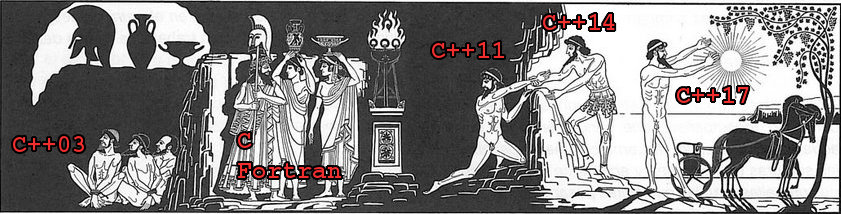
\includegraphics[width=\textwidth]{fig/cave}
    \vspace{1mm}
    \vspace{-3mm}
  \begin{itemize}
    \item Working code from examples on GitHub:
    \begin{itemize}
      \item \raisebox{-.08\height}{
\includegraphics[width=9px]{fig/github.pdf}}
            \url{https://github.com/ivankp/pgo_cxx}
    \end{itemize}
  \end{itemize}
}

% ===================================================================

\frame{\frametitle{Get a new compiler}
  % \toplink{http://mirrors.concertpass.com/gcc/releases/}
  \toplink{https://gcc.gnu.org/}
  \vspace{-3mm}
  \begin{itemize}
    \item \texttt{\ttc{bashkey}{wget} {\scriptsize\url{http://mirrors.concertpass.com/gcc/releases/gcc-6.3.0/gcc-6.3.0.tar.bz2}}}
    \item \texttt{\ttc{bashkey}{tar} xvjf gcc-6.3.0.tar.bz2}
    \item \texttt{\ttc{bashkey}{cd} gcc-6.3.0}
    \item \texttt{./contrib/download\_prerequisites}
    \item \texttt{\ttc{bashkey}{cd} ..}
    \item \texttt{\ttc{bashkey}{mkdir} build-gcc-6.3.0}
    \item \texttt{\ttc{bashkey}{cd} build-gcc-6.3.0}

    \item {\scriptsize\texttt{\ttc{bashval}{\$PWD}/../gcc-6.3.0/configure --prefix=\ttc{bashval}{\$HOME}/gcc-6.3.0 --enable-languages=c,c++,fortran --with-default-libstdcxx-abi=gcc4-compatible --enable-bootstrap --enable-threads=posix --with-long-double-128 --enable-long-long --enable-lto --enable-gnu-unique-object --enable-gold --with-system-zlib --disable-nls}}

    \item \texttt{\ttc{bashkey}{make} -j8}
    \item \texttt{\ttc{bashkey}{make} -j8 install}
  \end{itemize}
}

% ===================================================================
\newlength{\defaultlmii}
\setlength{\defaultlmii}{\leftmarginii}
\setlength{\leftmarginii}{12pt}

\frame{\frametitle{Get a new compiler}
  \begin{itemize}
    \item After installation is complete, you can remove \ttc{termdir}{build-gcc-6.3.0}.
    \item If you want to use the new compiler by default,\\
          only two environmental variables are needed
    \vspace{3mm}
    \begin{itemize}
      \item \texttt{\ttc{bashkey}{export} \ttc{bashvar}{PATH}=\ttc{bashval}{\$HOME}/gcc-6.3.0/bin:\ttc{bashval}{\$PATH}}
      \item \texttt{\ttc{bashkey}{export} \ttc{bashvar}{LD\_LIBRARY\_PATH}=\ttc{bashval}{\$HOME}/gcc-6.3.0/lib64:\ttc{bashval}{\$LD\_LIBRARY\_PATH}}
    \end{itemize}
    \vspace{3mm}
    \item Or you can just call the \texttt{g++} executable by the whole path.
    \item New headers and libraries are automatically looked up first during
      compilation and linking. No extra environmental variables needed.
    \item Setting \ttc{bashvar}{LD\_LIBRARY\_PATH} can be avoided by compiling
      with \texttt{-Wl,-rpath=\ttc{bashval}{\$HOME}/gcc-6.3.0/lib64}
  \end{itemize}
}

\setlength{\leftmarginii}{\defaultlmii}
% ===================================================================

\begin{frame}[fragile=singleslide]
\frametitle{Range-based for loop}
  \toplink{http://en.cppreference.com/w/cpp/language/range-for}

\vspace{-5mm}
Example 1:
\vspace{-3mm}
\begin{minted}[mathescape,fontsize=\footnotesize,frame=lines]{cpp}
for (int i : {1,3,5,7,9,11,13,17})
  cout << i << endl;
\end{minted}

\vspace{3mm}
Example 2:
\vspace{-3mm}
\begin{minted}[mathescape,fontsize=\footnotesize,frame=lines]{cpp}
std::vector<std::vector<TH1*>> hists;
. . .
for (auto& hh : hists)
  for (auto* h : hh)
    cout << h->GetName() << endl;
\end{minted}
\end{frame}

% ===================================================================

\begin{frame}[fragile=singleslide]
\frametitle{Range-based for loop}
  \toplink{http://en.cppreference.com/w/cpp/language/range-for}

\vspace{-5mm}
\textbf{How it works}
\begin{minted}[mathescape,fontsize=\footnotesize,frame=lines]{cpp}
std::vector<int> vec;
for (auto x : vec) { . . . }
\end{minted}

\vspace{2mm}
is equivalent to

\begin{minted}[mathescape,fontsize=\footnotesize,frame=lines]{cpp}
for (std::vector<int>::iterator it  = vec.begin,
                                end = vec.end();
     it!=end; ++it)
{
  int x = *it;
  . . .
}
\end{minted}
\end{frame}

% ===================================================================

\begin{frame}[fragile=singleslide]
\frametitle{$\lambda$ functions}
  \toplink{http://en.cppreference.com/w/cpp/language/lambda}
  
\begin{itemize}
    \item Write functions inline!
    \item Great with standard algorithms like \texttt{std::sort},
          \texttt{std::accumulate}, etc.
\end{itemize}

Example: find distribution with highest mean
\vspace{-3mm}
\begin{minted}[mathescape,fontsize=\footnotesize,frame=lines]{cpp}
std::vector<TH1D*> hists;
. . .
auto highest_mean = *std::max_element(
  hists.begin(), hists.end(), [](auto h, auto i) {
    return h->GetMean() < i->GetMean();
  }
);
\end{minted}

\end{frame}

% ===================================================================

\begin{frame}[fragile=singleslide]
\frametitle{$\lambda$ functions}
  \toplink{http://en.cppreference.com/w/cpp/language/lambda}

\begin{itemize}
  \item Capture variables from the environment in the \texttt{[]}.
\end{itemize}

Example: sort functions by their maxima or minima
\vspace{-3mm}
\begin{minted}[mathescape,fontsize=\footnotesize,frame=lines]{cpp}
std::vector<TF1*> funcs;
bool ascending;
. . .
std::sort(
  funcs.begin(), funcs.end(), [ascending](auto f, auto g) {
    double f_max = f->GetMaximum(),
           g_max = g->GetMaximum();
    return ascending ^ g_max < f_max;
  }
);
\end{minted}

\end{frame}

% ===================================================================
% https://www.sharelatex.com/learn/Code_Highlighting_with_minted

\begin{frame}[fragile=singleslide]
\frametitle{Variadic templates}
  \toplink{http://en.cppreference.com/w/cpp/language/parameter_pack}

\vspace{-5mm}
{\large$$\sum_ix_i^2$$}

\vspace{-5mm}
\begin{minted}[mathescape,fontsize=\footnotesize,frame=lines]{cpp}
template <typename T>
constexpr T sq(T x) noexcept { return x*x; }

template <typename T, typename... TT>
constexpr T sq(T x, TT... xx) noexcept { return sq(x)+sq(xx...); }
\end{minted}

\vspace{4mm}
Usage example:

\vspace{-4mm}
\begin{minted}[mathescape,fontsize=\footnotesize,frame=lines]{cpp}
double hypotenuse = std::sqrt(sq(3.,4.)); // 5
\end{minted}
\end{frame}

% ===================================================================

\begin{frame}[fragile=singleslide]
\frametitle{Variadic templates}
  \toplink{http://en.cppreference.com/w/cpp/language/parameter_pack}

\vspace{-5mm}
\begin{minted}[mathescape,fontsize=\footnotesize,frame=lines]{cpp}
#include <sstream>

template <typename S, typename T>
inline void cat_impl(S& ss, T&& x) {
  ss << std::forward<T>(x);
}

template <typename S, typename T, typename... TT>
inline void cat_impl(S& ss, T&& x, TT&&... xx) {
  ss << std::forward<T>(x);
  cat_impl(ss,std::forward<TT>(xx)...);
}

template <typename... TT>
inline std::string cat(TT&&... xx) {
  std::stringstream ss;
  cat_impl(ss,std::forward<TT>(xx)...);
  return ss.str();
}
\end{minted}
\end{frame}

% ===================================================================

\begin{frame}[fragile=singleslide]
\frametitle{Variadic templates}
  \toplink{http://en.cppreference.com/w/cpp/language/parameter_pack}

\vspace{-1mm}
Example 1:
\vspace{-3mm}
\begin{minted}[mathescape,fontsize=\footnotesize,frame=lines]{cpp}
cout << cat("char_array",' ',5,' ',std::fixed,std::setprecision(2),4.2)
     << endl; // char_array 5 4.20
\end{minted}

\vspace{2mm}
Example 2:
\vspace{-3mm}
\begin{minted}[mathescape,fontsize=\footnotesize,frame=lines]{cpp}
TFile file("file.root");

for (int j : {1,2,3}) {
  const auto name = cat("jet",j,"_pT");
  TH1 *hist = dynamic_cast<TH1*>(file->Get(name.c_str()));

  if (!hist) throw std::runtime_error(cat(
    name," histogram does not exists in file ",file.GetName()));

  if (hist->GetEntries()==0) throw std::runtime_error(cat(
    hist->GetName()," histogram is empty"));

  . . .
}
\end{minted}
\end{frame}

% ===================================================================

\begin{frame}[fragile=singleslide]
\frametitle{\texttt{C++17} fold expressions}
  \toplink{http://en.cppreference.com/w/cpp/language/fold}

\vspace{-5mm}
\begin{minted}[mathescape,fontsize=\footnotesize,frame=lines]{cpp}
template <typename... Args>
inline std::string cat(Args&&... args) {
  std::stringstream ss;
  (ss << ... << args); // fold expression
  return ss.str();
}
\end{minted}
\end{frame}

% ===================================================================

\begin{frame}[fragile=singleslide]
\frametitle{Smart pointers}
  \toplink{http://en.cppreference.com/w/cpp/memory}

\begin{itemize}
  \item These own dynamically allocated memory and clean it up automatically
        (\texttt{delete} called on destruction of pointer).
\end{itemize}

Example: distribution of a sample mean
\vspace{-3mm}
\begin{minted}[mathescape,fontsize=\footnotesize,frame=lines]{cpp}
std::random_device device;
std::mt19937 engine(device());
std::uniform_real_distribution<double> dist;

TH1::AddDirectory(false);
auto sample_mean = std::make_unique<TH1D>("sample_mean", "", 100, 0.0,
                                          1.0);
for (std::size_t i = 0; i < 1'000'000; ++i) {
  auto sample = std::make_unique<TH1D>("sample", "", 100, 0.0, 1.0);
  for (std::size_t j = 0; j < 10; ++j) sample->Fill(dist(engine));
  sample_mean->Fill(sample->GetMean());
}
\end{minted}

\end{frame}

% ===================================================================

\begin{frame}[fragile=singleslide]
\frametitle{Uniform initialization}
  \toplink{http://en.cppreference.com/w/cpp/language/aggregate_initialization}

\vspace{-5mm}
\begin{minted}[mathescape,fontsize=\footnotesize,frame=lines]{cpp}
struct point { double x, y; }; // local class
std::vector<point> points {
  {0.1, 0.3},
  {3.1, 4,7},
  {55., 34.}
};

for (const auto& p : points)
  cout << '(' << p.x << ',' << p.y << ')' << endl;
\end{minted}
\end{frame}

% ===================================================================

\begin{frame}[fragile=singleslide]
\frametitle{\ttc{cpptype}{auto} and \ttc{cpptype}{decltype}}
  \toplink{http://en.cppreference.com/w/cpp/language/decltype}

\vspace{-5mm}
\begin{minted}[mathescape,fontsize=\footnotesize,frame=lines]{cpp}
std::vector<some_very_useful_but_very_long_type> vec;

auto it = vec.begin();

decltype(*it) x;
\end{minted}

\begin{itemize}
  \item The type of \texttt{it} is
    \texttt{std::vector<some\_very\_useful\_but\_very\_long\_type>::iterator};
  \item The type of \texttt{x} is
    \texttt{some\_very\_useful\_but\_very\_long\_type};
\end{itemize}

\end{frame}

% ===================================================================

\begin{frame}[fragile=singleslide]
\frametitle{Regular expressions}
  \toplink{http://en.cppreference.com/w/cpp/regex}

\vspace{-5mm}

Suppose you have histograms with name like
\begin{itemize}
  \footnotesize
  \item \texttt{jet1\_pT}
  \item \texttt{jet2\_pT}
  \item \texttt{jet1\_rapidity}
  \item \texttt{lepton2\_rapidity}
  \item \texttt{higgs\_pT}
  \item \texttt{higgs\_mass}
\end{itemize}
\vspace{3mm}

but you want to do something for only jet and Higgs pT histograms.

\begin{minted}[mathescape,fontsize=\footnotesize,frame=lines]{cpp}
std::regex re("(jet[0-9]|higgs)_pT");
for (TH1* h : hists) {
  if (std::regex_match( h->GetName(), re )) {
    . . . // Do something
  }
}
\end{minted}

\end{frame}

% ===================================================================

\begin{frame}[fragile=singleslide]
\frametitle{\texttt{<array>}}

\vspace{-5mm}

\texttt{std::array} is like \texttt{std::vector}, but statically allocated and
with the size a part of its type.

\begin{minted}[mathescape,fontsize=\footnotesize,frame=lines]{cpp}
using p4 = std::array<double,4>; // can use it to represent 4-momentum
std::vector<p4> particles; // will be contiguously allocated
\end{minted}

Other similar aggregate templates (statically allocated containers):
\begin{itemize}
  \item \texttt{std::pair<T1,T2>} -- 2 heterogenious types
    \href{http://en.cppreference.com/w/cpp/utility/pair}{
      \raisebox{-.08\height}{
\includegraphics[width=9px]{fig/link.pdf}}}
  \item \texttt{std::tuple<Ts...>} -- $n$ heterogenious types
    \href{http://en.cppreference.com/w/cpp/utility/tuple}{
      \raisebox{-.08\height}{
\includegraphics[width=9px]{fig/link.pdf}}}
  \item \texttt{std::array<T,N>} -- $n$ homogenious types
    \href{http://en.cppreference.com/w/cpp/container/array}{
      \raisebox{-.08\height}{
\includegraphics[width=9px]{fig/link.pdf}}}
\end{itemize}
\end{frame}

% ===================================================================

\begin{frame}[fragile=singleslide]
\frametitle{An analysis example}
  \toplink{https://github.com/ivankp/pgo_cxx/blob/master/src/analysis.cc}

\begin{itemize}
  \item An example of analysis code, reading a \texttt{TTree} from a ROOT file,
    making histograms of particle's transverse momentum for different types of
    events.
  \item Example of using \texttt{std::unordered\_map} and a timed counter based
    on \texttt{C++11} \texttt{<chrono>}.
  \item Also uses other previously discussed features.
\end{itemize}

\begin{center}
  \href{https://github.com/ivankp/pgo_cxx/blob/master/src/analysis.cc}
  {Link to the code}
\end{center}

\end{frame}

% ===================================================================

\begin{frame}[fragile=singleslide]
\frametitle{A fitting example}
  \toplink{https://github.com/ivankp/pgo_cxx/blob/master/src/minuit.cc}

\begin{itemize}
  \item An example of fitting code, using lambda functions with \texttt{TMinuit}.
  \item The
    \href{https://github.com/ivankp/pgo_cxx/blob/master/include/minuit.hh}{wrapper}
    for \texttt{TMinuit} also demonstrates other modern \texttt{C++} features.
\end{itemize}

\begin{center}
  \href{https://github.com/ivankp/pgo_cxx/blob/master/src/minuit.cc}
  {Link to the code}
\end{center}

\end{frame}

% ===================================================================

\begin{frame}[fragile=singleslide]
\frametitle{Move semantics}
  \toplink{http://en.cppreference.com/w/cpp/language/move_constructor}

\begin{itemize}
  \item Prevents unnecessary copying of dynamically allocated memory.
  \item Compiling with \texttt{-std=c++11} or later turns these on
        automatically in the standard library.
\end{itemize}

Example: return a \texttt{std::vector} from a function
\vspace{-3mm}
\begin{minted}[mathescape,fontsize=\footnotesize,frame=lines]{cpp}
std::vector<double> sample_dist(std::size_t n_samples) {
  . . .
}

int main() {
  auto samples = sample_dist(1000000);
  . . .
}
\end{minted}

\end{frame}

% ===================================================================

\end{document}
